\documentclass[article]{jss}

%% -- LaTeX packages and custom commands ---------------------------------------

%% recommended packages
\usepackage{thumbpdf,lmodern}

%% another package (only for this demo article)
\usepackage{framed}
\usepackage{float} %for figure [H]
%% new custom commands
\newcommand{\class}[1]{`\code{#1}'}
\newcommand{\fct}[1]{\code{#1()}}
\newcommand{\imgdir}{../../../paperImage/}
%% For Sweave-based articles about R packages:
%% need no \usepackage{Sweave}
%\SweaveOpts{engine=R, eps=FALSE, keep.source = TRUE}


%% -- Article metainformation (author, title, ...) -----------------------------

%% - \author{} with primary affiliation
%% - \Plainauthor{} without affiliations
%% - Separate authors by \And or \AND (in \author) or by comma (in \Plainauthor).
%% - \AND starts a new line, \And does not.
\author{Bo-Syue Jiang\\National Taipei University
\And Han-Ming Wu\\National Chengchi University}
\Plainauthor{Bo-Syue Jiang,Han-Ming Wu}

%% - \title{} in title case
%% - \Plaintitle{} without LaTeX markup (if any)
%% - \Shorttitle{} with LaTeX markup (if any), used as running title
\title{ggESDA: An \proglang{R} Package for Exploratory Symbolic Data Analysis using \pkg{ggplot2}}
\Plaintitle{A Short Demo Article: Regression Models for Count Data in R}
\Shorttitle{A Short Demo Article in \proglang{R}}

%% - \Abstract{} almost as usual
\Abstract{
  This paper presents the \pkg{ggESDA} package, which we developed for exploratory symbolic data analysis in \proglang{R}. Based on \pkg{ggplot2} \cite{Wickham:2009}, the \pkg{ggESDA} package which is familiar programming structure with its parent provides a wide variety of graphical techniques such as histogram, 3D-scatterplot and radar plot. In addition, a general and  customized transformation function \code{classic2sym()} is implemented for generating a symbolic data table from classical data frame by clustering algorithm, \pkg{RSDA} \cite{Rojas:2015} function and user-defined method. wait for edit......
}

%% - \Keywords{} with LaTeX markup, at least one required
%% - \Plainkeywords{} without LaTeX markup (if necessary)
%% - Should be comma-separated and in sentence case.
\Keywords{data visualization, symbolic data analysis, exploratory data analysis, \pkg{ggplot2} extensions, interval-valued data, \proglang{R}}
\Plainkeywords{data visualization, symbolic data analysis, exploratory data analysis, ggplot2 extensions, interval-valued data, R}

%% - \Address{} of at least one author
%% - May contain multiple affiliations for each author
%%   (in extra lines, separated by \emph{and}\\).
%% - May contain multiple authors for the same affiliation
%%   (in the same first line, separated by comma).




\begin{document}
%\SweaveOpts{concordance=TRUE} 
\section{Introduction}
"In Data Science the aim is to extract new knowledge from Standard, Big, and complex data. Often these data are unstructured with variables defined on different kinds of units. They can also be multi-sources (as mixtures of numerical and textual data, with images and networks)." \cite{Diday:2018}. The statement indicates that not only conventional data but the unstructured data, also known as symbolic data, is vital for data science. Rather than the classical data represented by a single value, symbolic data with measurements on $p$ random variables can be $p$-dimensional statistical units such as hypercubes or histograms. The field of symbolic data analysis (SDA) \cite{Billard+Diday:2007} is to broaden the application aspects of statistical methodologies, extend traditional cognition of a form of data unit and build a brand-new analysis system of data science. Recent developments in the field of big data analytics have led to a renewed interest in complex structure data such as symbolic data. As shown in Figure \ref{fig:trend}, the number of researches in SDA represents an increasing trend from 1998 to 2020, which outstands the importance of it during the years.
\begin{figure}[h]	
  		\centering	 			 	 
 	 		\includegraphics[width=1\textwidth]{\imgdir Trend_SDA_1998_to_2020.png} 
  		\caption{The number of "symbolic data analysis" or "interval-valued data" related articles in researches and applications according to PubMed and ScienceDirect online database over time from 1998 to 2020.}   		
  		\label{fig:trend}   			 		 
\end{figure}
Among ScienceDirect, Engineering and Computer Science lead the subject areas obviously, shown in Figure \ref{fig:subjectAreas}.
\begin{figure}[h]	
  		\centering	 			 	 
 	 		\includegraphics[width=1\textwidth]{\imgdir subjectAreas_scienceDirect.png} 
  		\caption{Top 10 researches and applications domains for SDA or interval-valued data (ScienceDirect) from 1998 to 2020} 
  		\label{fig:subjectAreas}   			 		 
\end{figure}


In practice, the symbolic data is often generated by aggregating massive datasets into intervals in order to make the management easy and appropriate. An interval-valued symbolic random variable $X$, taking values in interval, can be denoted such as $X = [a,b] \subset  R^{1}$, where $a \leq b$, and $a, b \in R^{1}$. Let the random variable $X$, for instance, be the weight, then $X = [50,100]$ represents the interval covering the weight of people. With the advent of big data analytic, interval-valued data is becoming more common and accessible than ever. The researches for interval-valued data such as the sign test for COVID-19 data \cite{sherwani:2021}, the prediction via regularized artificial neural network \cite{yang:2019}, a bivariate Bayesian method for regression models \cite{xu:2021}, etc.

Exploratory Data Analysis (EDA) \cite{Tukey:1977} is primarily used to see what data can reveal beyond the formal modeling or hypothesis testing task, provides an overview of raw datasets and obtains a general understanding about the variables and their relationships.


\section{Prominent SDA packages}

\subsection[RSDA]{\pkg{RSDA}}

\subsection[symbolicDA]{\pkg{symbolicDA}}

\subsection[HistDAWass]{\pkg{HistDAWass}}




\section[Basic usage of ggESDA]{Basic usage of \pkg{ggESDA}}

\pkg{ggESDA} is now available from the Github at \url{https://github.com/kiangkiangkiang/ggESDA}. All reference manual documented by exported functions and introduction vignettes can also be download here. In the following section, we are going to illustrate the functionalities and syntaxes about \pkg{ggESDA}.

\subsection[Transformation function]







\subsection{General principles}

\subsection{Multiple plot}

\subsection{Package dependencies}


\section{Application to real datasets}

\subsection{univariate}

\subsection{bivariate}

\subsection{multivariate}


\section{Conclusion}



\section{why SDA plot (weakness of classical plot)}
\subsection{sol overstike}
For the conventional exploratory data analysis, it is always a severe challenge to deal with enormous datasets because conventional displays suffered from overstrikes of data points representing the value (scatterplot type displays) or overstrikes of line segments connecting values of neighboring variables. As a consequence, exploratory symbolic data analysis (SDA) becomes a preliminary yet essential tool for summarizing the main characteristics of a data set before appropriate statistical modeling can be applied. Besides escaping the problem mentioned above, SDA can effectively reduce observations in data, which will make the study focus on what we interesting instead of unnecessary information such as Figure~\ref{fig:compare}.

\begin{figure}[H]
\centering
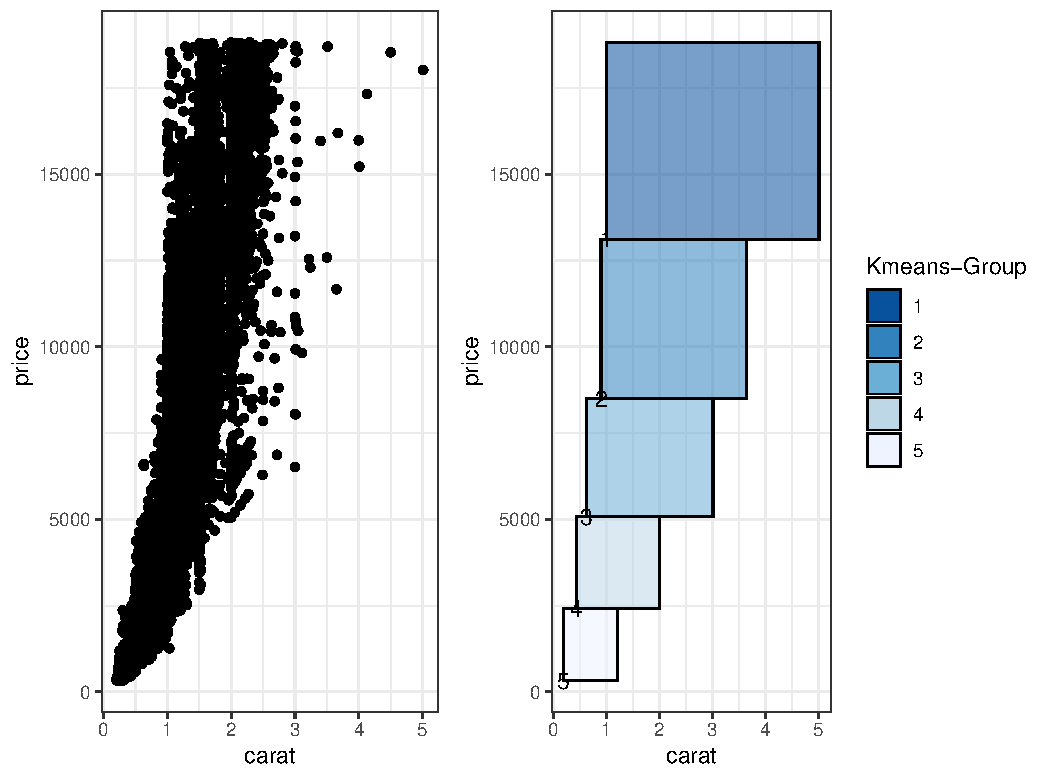
\includegraphics{ggESDA_Jiang&Wu_20210915-compare}
\caption{\label{fig:compare} Compare classical data and symbolic data}
\end{figure}

In Figure~\ref{fig:compare}, we can clearly visualize the scatter plot in the right hands, which is represented by symbolic data and aggregated by K-means \cite{Jin:2010}. 


\subsection{full information}

In the past, we would like to use barplot to visualize the frequency of categorical data, but that was merely represented the distribution of full data in that category. It cannot lead researchers to explore more details in what they are interesting such as a particular part of data, so aggregation methods play a vital role to merge the data we interesting.

However, the conventional categorical data after merging will usually be represented by mode, which will be unmeaningful to visualize and cause the loss of information that may become larger when the data or the number of factors in that category is growing on. SDA will build a histogram by calculating each factor of the category of frequency as bins to solve this kind of problem as a result. In that way, a categorical variable will never be shown as a single value at all, instead, a complete information histogram will be substituted.





\subsection{flexible coordinate}




\bibliography{refs}






\end{document}
